% The LaTeX template for the master's thesis 
% Degree Program: Computational Engineering and Technical Physics (LATE)
% University: LUT University, Finland
% Date: October 14, 2020

\documentclass{lutmscthesis}[2017/10/03]

\usepackage[utf8]{inputenc}
\usepackage[T1]{fontenc}
\usepackage[english]{babel}

\usepackage{times}
\usepackage{tabularx}
\usepackage{multirow}

\usepackage{setspace}
\usepackage{verbatim}
\usepackage[intlimits]{amsmath}
\usepackage{enumitem}

% The abbreviations
\usepackage[acronym,nomain,nonumberlist]{glossaries}
\makeglossaries
\newacronym{2d}{2-D}{two-dimensional}
\newacronym{nhl}{NHL}{National Hockey League}
\newacronym{ppv}{PPV}{Positive Predictive Value}
\newacronym{tp}{TP}{True Positive}
\newacronym{fp}{FP}{False Positive}

\usepackage{pgfplots} 
\pgfplotsset{compat=newest} 
\newlength\figurewidth
\newlength\figureheight

\usepackage{float}
\floatstyle{plain}\restylefloat{figure}
\floatstyle{plaintop}\restylefloat{table}

\usepackage[pdfborder={0 0 0}]{hyperref}
\usepackage[]{algorithm}
\usepackage{cite}

\usepackage[figure,table]{totalcount}

\graphicspath{{resources/}}

\newcommand{\vect}[1]{\boldsymbol{#1}}
\newcommand{\matr}[1]{\boldsymbol{#1}}
\newcommand{\diag}[1]{\mathrm{diag}(#1)}
\newcommand{\iprod}[1]{\left\langle #1 \right\rangle}
\newcommand{\me}{\mathrm{e}}
\newcommand{\mi}{\mathrm{i}}
\newcommand{\md}{\mathrm{d}}
\newcommand{\sse}{{}} %\mathrm{SSE}}
\newcommand{\trace}{\mathrm{Tr}\:}
\newcommand{\frp}[2]{{}^\mathrm{#1}\vect{#2}}
\newcommand{\frs}[3]{{}^\mathrm{#1}#2_\mathrm{#3}}
\newcommand{\frv}[3]{{}^\mathrm{#1}\vect{#2}_\mathrm{#3}}
\newcommand{\frm}[3]{{}^\mathrm{#1}\matr{#2}_\mathrm{#3}}
\newcommand{\colvec}[2]{\genfrac{[}{]}{0pt}{1}{#1}{#2}}
\newcommand{\relphantom}[1]{\mathrel{\phantom{#1}}}
\newcommand\aug{\fboxsep=-\fboxrule\!\!\!\fbox{\strut}\!\!\!}

\newcommand{\etal}{\textit{et al}. }

\newtheorem{theorem}{Theorem}

% Thesis information

\title{Practical Assignment Report}

\author{Tornike Onoprishvili, Aleksandr Algasov}

%\Major{Computer Vision and Pattern Recognition}

\Keywords{computer vision, machine vision, image processing, pattern recognition}

% Your supervision team

% \Supervisors{M.Sc. Donald Duck \\ Dr. . Kristian Superman \\ Adjunct Professor, Dr. Susan Wonderwoman\\ Professor Heikki K\"alvi\"ainen}

% The official examiners of your thesis

% \Examiners{Professor Heikki K\"alvi\"ainen \\ Adjunct Professor, Dr. Susan Wonderwoman}

\Year{2024}

% Thesis statistics for the abstract: number of pages, figures, tables, and appendices.

\addtostats{, 2 figures, 1 table, 2 appendices}

\begin{document}
\selectlanguage{english}

\maketitle
\newpage

\begin{abstract}

This is the abstract of the LaTeX template. The template contains a lot of writing instructions. 
This page is an abstract in English (Page 2).
Only the Finnish speaking students need to write also the abstract in Finnish (Page 3).
Present here the main items of your thesis: background, objectives, delimitations, results, and the main conclusions. 
Remember that the reader should be able to understand the abstract as it is. 
So there should not be any references or any need to read something else. 
Prefer short sentences and motive the reader to become interested in your work. 
Remember also that the abstract is separate from the rest of your thesis. 
So, for example, you should not assume that the abstract is a part of the introduction chapter, or vice versa.
The length of the abstract page is one page only so it should fit to one page (this page).
Moreover, the abstract text is one paragraph only, not two or many paragraphs. 
Use the passive form instead of the active form in the presentation, such as “this study focuses on intelligent computing applications”, not as “I studied intelligent computing applications” or “We studied intelligent computing applications”.

\end{abstract}


\begin{preface}

The author can decide the contents of this page. Usually the place of work and related people (supervisors, collaborators, friends, relatives, etc.) are acknowledged.

I would like to thank my supervisors ...friends ... family ...

Lappeenranta, \today

\end{preface}


% These name-definitions must be after Babel language change
% commands, as they redefine these.

\renewcommand\refname{REFERENCES}
\renewcommand\contentsname{CONTENTS}

\pagestyle{masters}
\newpage


% ---------------------------------------
%           TABLE OF CONTENTS
% ---------------------------------------

\tableofcontents


% ---------------------------------------
%    LIST OF SYMBOLS AND ABBREVIATIONS
% ---------------------------------------

\glsnogroupskiptrue
\setlength{\glsdescwidth}{1.0\hsize}
\printglossary[title=LIST OF ABBREVIATIONS,type=\acronymtype, style=long, nonumberlist, nopostdot]

Advice: All symbols and abbreviations are listed on this page in the alphabetical order. 
Remember to introduce the abbreviation when it is used in the text for the first time.\\

You may use the automated system, depending on your LaTeX environment:
\begin{verbatim}
\glsnogroupskiptrue
\setlength{\glsdescwidth}{1.0\hsize}
\printglossary[title=LIST OF ABBREVIATIONS,type=\acronymtype, 
style=long, nonumberlist, nopostdot]
\end{verbatim}

% Adding manually
%\section*{LIST OF ABBREVIATIONS}
%
%\begin{tabular}{l l}
%2-D & two-dimensional\\
%NHL & National Hockey League\\
%\vdots&\\
%\end{tabular}\\

% space between paragraphs
\setlength{\parskip}{3ex}


% ---------------------------------------
%             INTRODUCTION
% ---------------------------------------

\section{INTRODUCTION}
\label{sec:introduction}

\subsection{Background}
\label{sec:background}

This is the beginning of the LaTeX template for the text body. 
The template contains the main instructions for writing your thesis. 

Introduce the background of your thesis here: {\bf what, where, why, and how?}
Try to be compact and clear. 1-2 pages is enough for Chapter~\ref{sec:introduction}. 
It might be useful to show a figure here or in Section~\ref{sec:objectives} about the problem to be solved. 

The goal of this document is to be the template for your master's thesis, giving the instructions in writing and presenting your work. 
For further information, discuss with your supervisors, and visit the appropriate course web pages. 
When referring to web pages, do not use footnotes or do not write URLs within the text but give references. 
For example, saying that more information can be found as in the LUT study portal~\cite{lutstudyportal}.

Remember that the abstract is a separate piece of text. 
The introduction should be written independently such that the abstract is not needed to be read to understand the introduction. 
The introduction should be written such that the reader becomes interested to continue to read the full thesis. 
The introduction is written at the general level, instead of many details present. 
More details can be explained later starting from Chapter 2. 

More hints about writing are presented as follows (still more hints to come later): 
\vspace{-18pt}
\begin{itemize}
\itemsep=-3pt
\item First of all, think first what you write more than directly write what you think. 
\item Avoid using “has/have” when the subject is not a living thing: “the page contains,” not “the page has,” etc. 
\item Do not use the future tense (will/shall) when you mean the present tense or would/should/could. Using the future tense means that you are sure that something will be done, but it has not yet been done. 
\item The paragraphs should contain more than one sentence only. Avoid too short paragraphs. 
\item Remember to introduce the abbreviations when they are used in the text for the first time. For example, ”This thesis is about the games played in \gls{nhl} in seasons 1900-2000. The annual penalties in~\gls{nhl} have … “. 
This is simple by using the automated introduction of the abbreviations offered by LaTeX. 
\item Check the layout before publishing your thesis. A section headline should not be the last line of the page. There should not be unnecessary empty space on the bottom of a page due to the insufficient layout of figures and tables.
\end{itemize}


\subsection{Objectives and delimitations}
\label{sec:objectives}

In this chapter, express the objectives of your work, including also the delimitations. 1-2 pages is enough. 

Tell what you are exactly going to do, and what you are not going to do. The best way is to formulate the objectives as research questions, or at least as clearly defined tasks, usually as a list: 
\begin{enumerate}
\item Is it possible to detect automatically traffic signs based real-time video processing? 
\item Can the condition of traffic signs be analyzed accurately enough? 
\item ...
\end{enumerate}

Alternatively, the objectives of the thesis are as follows:
\begin{itemize}
\item Automatic detection of traffic signs based real-time video processing. 
\item Condition analysis of traffic signs.  
\item ...
\end{itemize}

This way it is later easier to discuss later how the objectives were fulfilled. It is very important to define the objectives carefully so agree with your supervisors about the objectives.  

\subsection{Structure of the thesis}

This subsection contains a short description for the contents of the thesis. 
The contents of each chapter are characterized with one or two sentences. 
For example, "The state-of-the-art methods of edge detection are introduced in Chapter~\ref{sec:related}... Finally, in Chapter~\ref{sec:conclusion} the conclusions are given." 
Note that the main sections are referred as Chapters and subsections as Sections.

This subsection occupies at most one page, in many cases half a page is enough. At this point, one should thoroughly consider the structure of your work. Discuss with your supervisor about the structure.  

\section{RELATED WORK}
\label{sec:related}

Agree about the title of the chapter and the needed subsections with your supervisors. 
You may need to write more than one chapter only. 

The next subsections are for learning important details of writing the thesis. 

\subsection{References}

Find the related work by searching information sources. 
So your task is to find relevant information (example citations in parentheses): 
journal articles~\cite{hamouz2005feature}, 
conference paper~\cite{zafari2017comparison}, 
books~\cite{GonWoo:2002}, 
master theses~\cite{Lyubanenko2017MScThesis} and doctoral theses~\cite{strokina2013phdthesis}, 
web pages~\cite{lutstudyportal}, 
and other information.

Notice each publication type has the BibTex template of its own. See BibTex file for further information. 

It is important that in the list of references (called References) in your thesis you give all bibliographical information correctly and completely. So tell exactly what journal, conference, book, etc. in order to define the publication forum correctly. Distributors of publications like ResearchGate and IEEE Digital Library are not publishers to be mentioned, instead of original publication forums.

An example is given as follows:

Correct:\\
Zafari, S., Eerola, T., Sampo, J., Kälviäinen, H., Haario, H., Segmentation of Overlapping Elliptical Objects in Silhouette Images, IEEE Transactions on Image Processing, Vol. 24, No. 12, 2015, pp. 5942-5952.

Incorrect:\\
Zafari, S., Eerola, T., Sampo, J., Kälviäinen, H., Haario, H., Segmentation of Overlapping Elliptical Objects in Silhouette Images, ResearchGate, 2016. 

Write all your references on the references page with {\bf the full bibliographical details}: 
\vspace{-18pt}
\begin{itemize}
\itemsep=-4pt
\item All the names of the authors. 
\item The full title.
\item The full name of the publication forum. 
\item The publication details: volume, number, year, pages. 
\end{itemize}

When you give the names of the authors in References write the all the names. However, when you refer in the text you can write "Hamouz et al.~\cite{hamouz2005feature} proposed a method ..". In case of two authors only, write the both names. 

You can decide the style to present the publication details, but remember to use always the same style.

Do {\bf not} write the name of the publication forum in the wrong order as \\
Image Processing, IEEE Transactions on\\
or using partly abbreviations as\\
Int J Comp Vision.

\subsection{Chapters and sections}

Divide your chapter into suitable subsections. You may need to have several chapters for presenting related work, 
especially if you have a certain application field or you focus on a subset of methods.

See the following examples: 

1. Introduction\\
1.1 Background\\
1.2 Objectives and delimitations\\
1.3 Structure of the thesis\\
2. Road maintenance and inventory \\
2.1 Automatic traffic sign recognition\\
...\\
3. Methods for traffic signs\\
3.1 Image pre-processing\\
...\\

1. Introduction\\
1.1 Background\\
1.2 Objectives and delimitations\\
1.3 Structure of the thesis\\
2. Segmentation \\
2.1 Threshold-based segmentation\\
...\\
3. Co-segmentation methods \\
3.1 Co-segmentation by extanding single-image segmentation\\
...\\

\subsection{Numbering and citations}

Present tables, figures, algorithms, equations, and appendices as numbered. Then you refer to them later. 

All figures, tables, references, algorithms, and appendices must be numbered in the increasing order. 
They all must be cited in the text and they never should appear between a section headline and text body. 
For example, there cannot be figures which are not mentioned in the text, and a paragraph cannot begin with a figure or a table. 
Appendices~\ref{app:results1} and~\ref{app:results2} are shown as examples about how to present an appendix.  

Citing to figures can be done as follows:

”Gonzalez and Woods state~\cite{GonWoo:2002} 
that in digital imaging contrast enhancement may lead into higher dynamics 
as shown in Fig.~\ref{fig:contrast}.” 

If the figure is directly copied from source, e.g., from a scientific article or a book the source must be mentioned in the figure caption.  If the figure is modified based on source this source is mentioned in the text where the figure is cited. {\bf The figure itself comes after the citation} in the text. This means that the figure is mentioned in the text before the figure is presented. 
The figure is presented after the end of the paragraph where it is cited. The alignment of the figure and the caption is centered. 
The caption is always under the figure, and it introduces the subfigures too as shown in~\ref{fig:contrast}.

\begin{figure}[ht]
	\centering
	\subfloat[][]{
		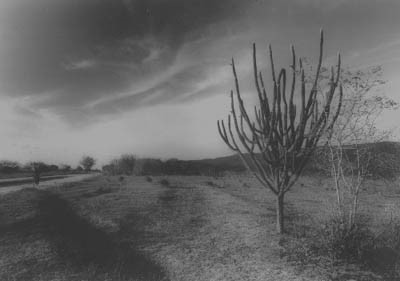
\includegraphics[width=0.40\linewidth]{resources/original.jpg}
		\label{subfig:original}
	}
	\subfloat[][]{
		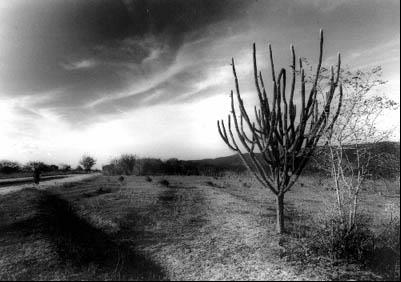
\includegraphics[width=0.40\linewidth]{resources/enhanced.jpg}
		\label{subfig:enhanced}
	}

 \caption[]{Contrast enhancement: 
\subref{subfig:original} 
Original image; 
~\subref{subfig:enhanced}
Enhanced image.~\cite{GonWoo:2002}}
\label{fig:contrast}
\end{figure}

The table caption is above the table as shown in Table~\ref{tab:grading}. 
The table and caption are aligned in the center. 
The table caption may contain more than one sentence. 
The texts in the figure caption and in the table caption always end with the period (the symbol "."). 

\begin{table}[ht]
\caption{Scaling for grading.}
\vspace{-12pt}
\begin{center}
\begin{tabular}{|l|c|c|c|c|c|c|}
\hline
Points &1--14 & 15--17 & 18--20 & 21--23 & 24--26 & 27--30\\
\hline
Grade &0&1&2&3&4&5\\
\hline
\end{tabular}
\label{tab:grading}
\end{center}
\end{table}

Figure and table captions must appear as full on one page. 
Thus, do not split them over several pages. 
For example, Fig.~\ref{fig:contrast} and Table~\ref{fig:contrast} including captions must be on one page only. 
Figures and tables are placed such that there is no extra empty space above or below them. 
Normally, figures and tables are placed on top of the page or on the bottom of the page, 
but they may appear also in the middle. 
If the figure or the table cannot be placed on the same page as the paragraph 
where they are cited then place the figure and the table on the next page. 
In this case the bottom of the page is filled with the text from the next paragraph.  
Thus, do not generate half empty pages. 

Equations are always numbered and they must be a part of sentences in the text. 
Thus, the presentation should not be disconnected because of an equation. 
Here it is presented an example how to include an equation in the text~\cite{zafari2017comparison}:  

The concavity value of $c_{d,i}$ is defined as the angle between lines $(c_{d,i-1} , c_{d,i} )$ and $(c_{d,i+1} , c_{d,i})$ as follows:
\begin{align}
\label{eq:value}
\begin{cases}
\mid a(c_{d,i-1} , c_{d,i} ) - a(c_{d,i+1} , c_{d,i} )\mid & \hspace{-5pt}\text{if}  \ |a(c_{d,i-1} , c_{d,i} ) - a(c_{d,i+1} , c_{d,i} )| < \pi\\
\pi  - |a(c_{d,i-1} , c_{d,i} ) - a(c_{d,i+1} ,c_{d,i})| & \hspace{-5pt} \text{otherwise} 
\end{cases}
\end{align}
where 
%$a(c_{d,i-1} , c_{d,i} )$ is the angle of line $\vec{c_{d,i-1} c_{d,i}}$ and
% $a(c_{d,i+1} , c_{d,i})$ is the angle of line
%$c_{d,i+1} , c_{d,i} $ as follows:
\begin{equation}
a(c_{d,i-1} , c_{d,i} ) = \tan^{-1} ((y_{d,i-1} - y_{d,i} )/(x_{d,i-1} - x_{d,i} ))
\label{eq:term1}
\end{equation}
and
\begin{equation}
a(c_{d,i+1} , c_{d,i}) = \tan ^{-1} ((y_{d,i+1} - y_{d,i} )/(x_{d,i+1} - x_{d,i} )).
\end{equation}

Then it is possible to refer to the first equation as Eq.~\ref{eq:value} and the second one as Eq.~\ref{eq:term1} later in the text. 

Another example is shown here how to present the equation: 

Correct:\\
Given a point $(x,y)$ a line can be presented as 
\begin{equation}
y = ax + b
\label{eq:line1}
\end{equation}
where $a$ and $b$ are line parameters. 

Incorrect:\\ 
Given a point $(x,y)$ a line can be presented.  
\begin{equation}
y = ax + b.
\label{eq:line2}
\end{equation}

In the latter case  the sentence has been ended by the period before Eq.~\ref{eq:line2}, 
and $a$ and $b$ have not been introduced. 
Remember that the period really ends the sentence. 

\section{PROPOSED METHODS}
\label{sec:proposed}

Agree about the subsections of this chapter with your supervisors.

\subsection{Algorithms}

In the thesis, there is at least one chapter about proposed work by the author and his collaborators. 
This can consist of new methods, frameworks, and software which are compared to the existing state-of-the-art solutions. 
Experimental comparisons are shown later in Chapter~\ref{sec:experiments}.
So here it is more like comparisons of characteristics, including method parameters. 

Present your developed methods in this chapter. 
Preferably show them step by step as algorithms where you clearly define method parameters, including input and output. 

An example is shown in Algorithm~\ref{alg:3d_reconstruction}. 
In our example, an important method parameter is t which defines 
how strong the intensity value of an edge pixel should be to be considered in a binarized edge image. 
One way is the top-down approach where you plan your algorithm at the high level and then begin to add detailed information. 
This can be one by extending one algorithm, by adding more steps, or by referring to other algorithms which are presented separately. 

\begin{algorithm}[!ht]
  \caption{Binarized edge detection}
  \label{alg:3d_reconstruction}
\vspace{8pt}
Input: Gray-level image I(x,y)\\
\vspace{-8pt}\\
Output: Binarized edge image B(x,y)
  \begin{enumerate}
    \item Apply edge detection to I(x,y) to produce the edge intensity image E(x,y). 
    \item Select a threshold value t. 
    \item For each pixel (x,y) in E if E(x,y)>t then B(x,y)=255 else  B(x,y)=0. 
  \end{enumerate}
\end{algorithm}

It might be useful to present also state-of-the-art methods as algorithms in the previous chapters. 
This makes it easier to compare them to your solutions, and to apply them to your solution when they are parts of your algorithms. 
For example, you may use a known edge detection approach in Algorithm~\ref{alg:3d_reconstruction}.  

\subsection{Visual descriptions}

Another option is to illustrate your approach as show in Fig.~\ref{fig:framework}~\cite{norppa2017}.

\begin{figure}[ht]
\begin{center}
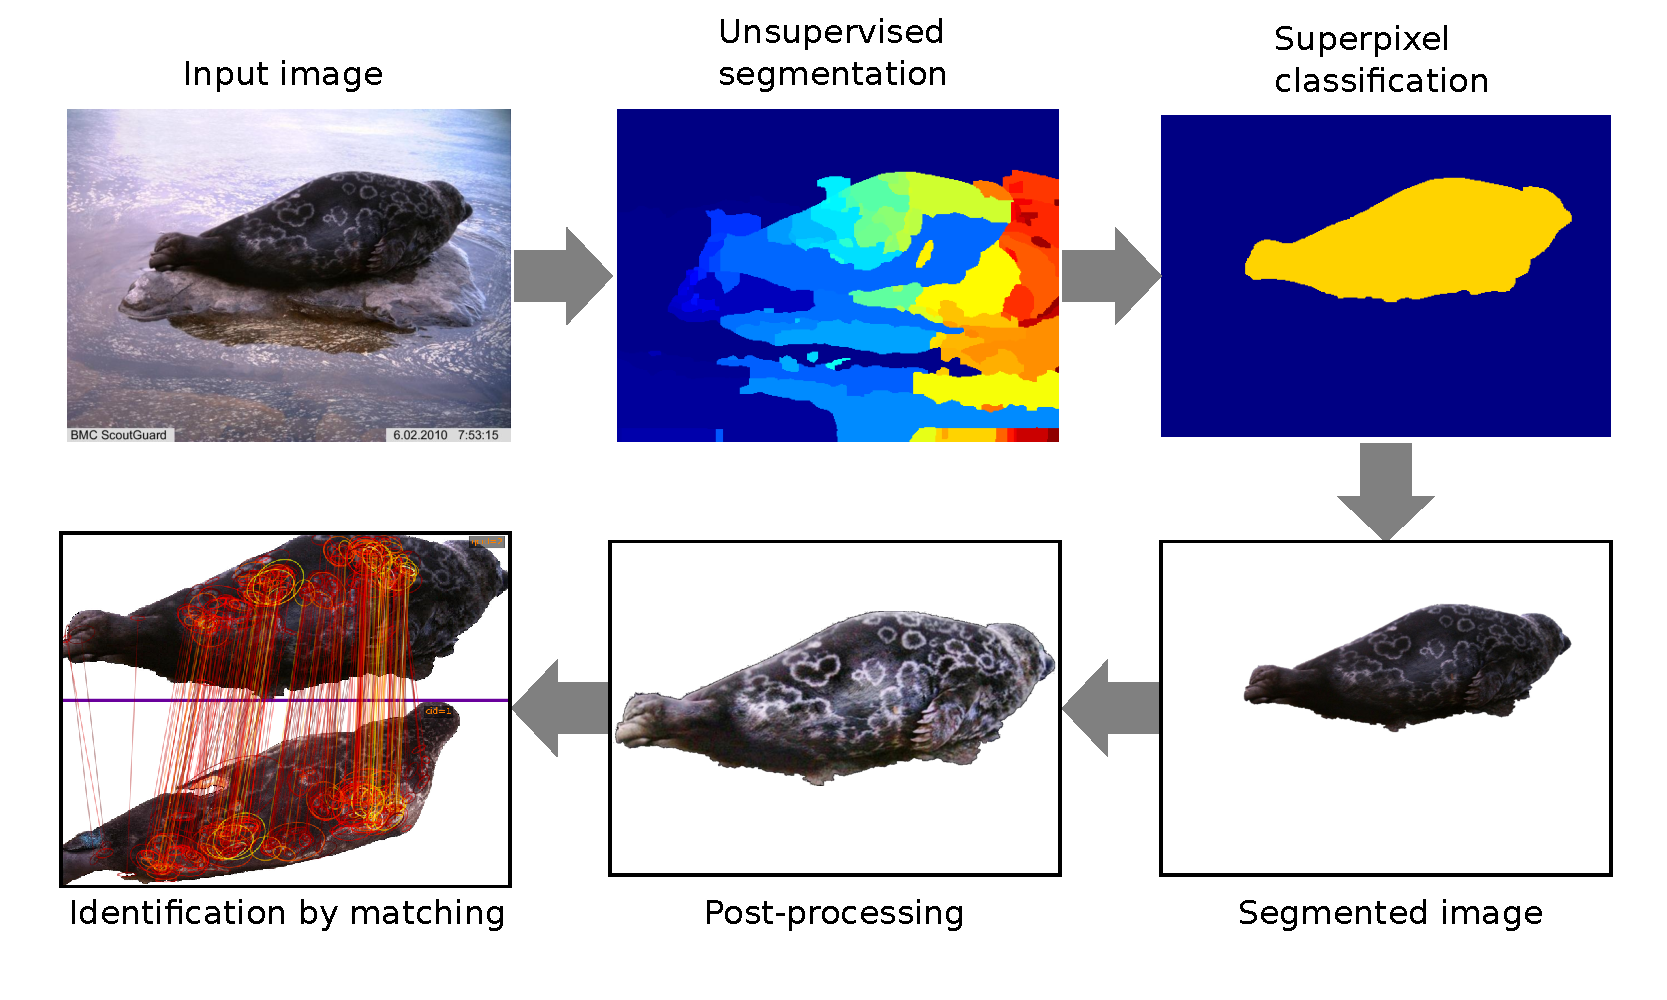
\includegraphics[width=\textwidth]{resources/framework.pdf}
\caption{The proposed method for the identification of Saimaa ringed seals.~\cite{norppa2017}} \label{fig:framework}
\end{center}
\end{figure}

\section{EXPERIMENTS}
\label{sec:experiments}

\subsection{Data}

Introduce your data here. If you have many datasets name them. For example, Dataset 1 consists of 100 gray-level images and Dataset 2 consists 150 color images. The images present \gls{2d} objects.  

\subsection{Evaluation criteria}

Tell how you evaluate the quality of your experiments. Define your evaluation criteria. 

For example, the text could be like as follows:

To evaluate the method performance and to compare the methods, 
\gls{ppv} was used and is defined as follows:
\begin{equation}
PPV = \frac{TP}{TP+FP}
\end{equation}
where \gls{tp} is the number of the correctly detected objects and 
\gls{fp} is the number of the incorrectly detected objects.
 
\subsection{Description of experiments}

Describe your experiments. If you have many name them as needed. For example, Experiment 1 (or Experiment A) and Experiment 2 (or Experiment B). 

Tell the details: what data (the training set and the test set) and what methods. For example, in Experiment 1, Dataset 1 was divided at random to the training set of 50 images and the test set of 50 images, and was tested with Methods A, B, and C. 

\subsection{Results}

Show and explain your results. Remember to study parameter sensitivity, i.e., how sensitive each method is to the selection of parameters. 

Remember to explain the axes of figures and the headings of tables. Moreover, use the same and reasonable numeric presentation of the results. For example, decide how many decimals are needed. 

\section{DISCUSSION}
\label{sec:discussion}

\subsection{Current study}

This chapter analyzes the results further, leading to conclusions with reasonable arguments. 
The research questions (tasks) defined in the introduction should be considered in this chapter. 
In the last chapter (Chapter~\ref{sec:conclusion}) there is only a compact summary of conclusions made earlier 
so all reasoning should happen at latest in the discussion chapter. 
Remember to clearly tell what are your contributions, 
the contributions of your collaborators, and the contributions of the others. 

\subsection{Future work}

Discuss about the future study needed.

\section{CONCLUSION}
\label{sec:conclusion}

The last chapter of the work is the conclusion. 
This section summarizes work done, including the results and the conclusions from the results, 
based on discussions in the previous chapters. 
There should not be anything new given in this chapter: 
no new conclusions neither new proposals for the future work.
The presentation is usually very compact and straightforward to read, 
the length of the page being at maximum one page.   
 
\clearpage

% Bibliography
% The name of the BibTeX file is given here. 
% Make sure that your BibTeX file contains all needed bibliographical details. 

\addcontentsline{toc}{section}{REFERENCES}
\bibliography{resources/thesis}


%% ----------------------- APPENDICES ------------------------------

\appendix
 
\section{Results from the first experiment.}
\label{app:results1}

For example, you can present more detailed results of your experiments here. 

\newpage 

\section{Results from the second experiment.}
\label{app:results2}

For example, you can present more detailed results of your experiments here.

\end{document}
